\chapter{Methodology}\label{chap_methodology}
% This section will depend on the fundamental research you are undertaking, for example, if you are undertaking a purely experimental study you would be expected to indicate the materials and equipment/instruments used, as well as experimental methods. You may wish to use diagrams or figures if appropriate. 

% For a purely computational study you would be expected to report the operating system, methods, software, parameters etc. used in your study. Again diagrams or figures may be useful. Some studies may contain a mixture of computational and experimental methods. These should both be included.

% Within the methodology section, you should describe concisely exactly how the investigation was carried out, with enough detail to allow the study to be replicated.

% The report should be written in a scientific format e.g. Samples containing 1.0, 0.1, 0.01 % (w/v) element X were measured using instrument Y, at room temperature (22°C). Results were analysed using software Z, applying the following parameters…

The methodology used is to perform numerical simulation (\textit{Computational Fluid Dynamics}, CFD) using 
an in-House high order Fortran90 code, the complex data structure of this code requires a careful reading of its source file, in particular taking confidence is needed in the input parameters and the output in order to be able to manage the simulation (changing some boundary condition value or restarting simulation from a certain point), and well interpreting the output.  %understanding of the source file.
This requires an indispensable spend of time, and one years of usage may not be enough to have completely confidence 
with the code.

\section{Realizing valutable output}

When we deal with numerical simulation, one of the most important things is the post-processing of the result,
to present them clearly and understandably. For this pourpose the first thing was to develop a program written in C++ and in Fortran to convert the data file containing the cordinate of the beads~\cite{pp} 
of the polymer in a format readable from the software for visualizing the chains represented from separated beans connected from a spring. This is the so called \textit{beads-spring model}~\cite{pp} 
for studying the polymer chains. The Visualisation tool used is the free and open-source code PARAVIEW that reads the file in several format, but the much more indicated is the format VTK. This allows to visualize the polymer chains as reported in figure~\ref{fig:chains}

\begin{figure}[h]
\centering
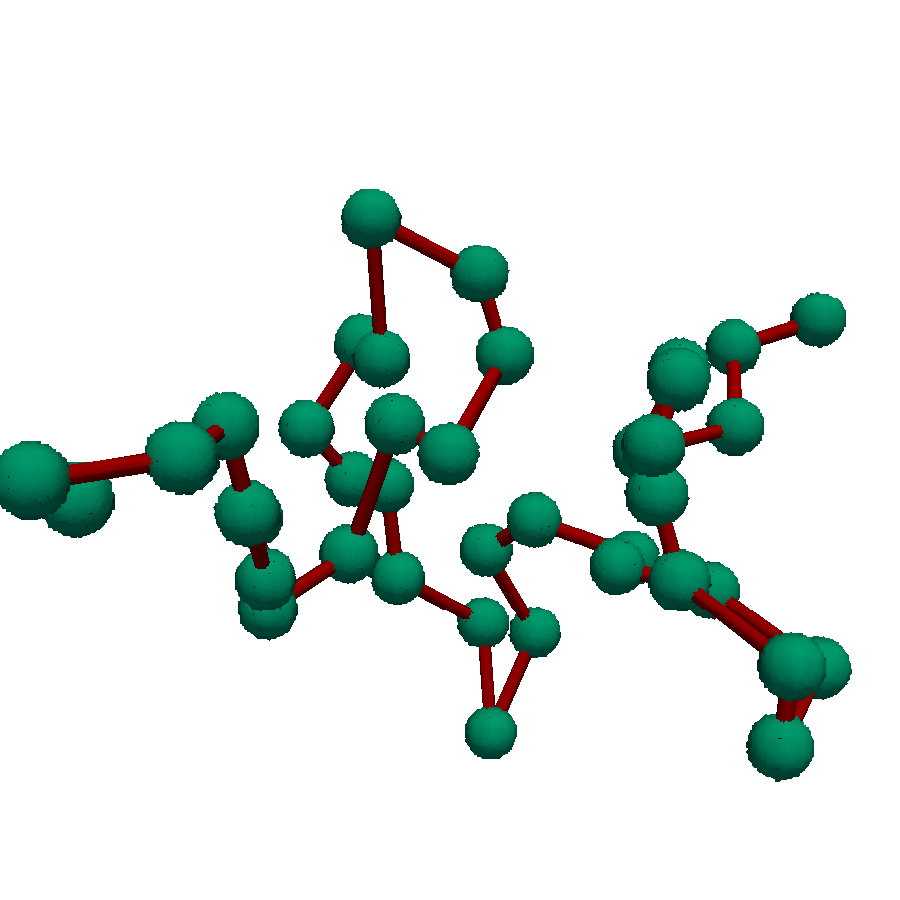
\includegraphics[width=.4\textwidth]{chain.png} 
\caption{Polymer chains post processing with PARAVIEW}
\label{fig:chains}
\end{figure}

In order to develop this program, a deep knowledge of the VTK C++ library is needed. 
The tool developed was useful to postprocess the vorticity and velocity field that surrounds 
the polymer chain

\section{Numerical Modelling}

As already said the aims of this Ph.D is to investigate the behaviour of polymer chains surrounding from the 
turbulent velocity field of the solvent. 

Hydrodynamic interaction between solvent and polymer chains are computed using:
\begin{itemize}
\item A Coarsed Grained Molecular Dynamic, \textsc{langevin equation}, for the polymer chain. 

\item The turbulent fluid field is governed by the \textsc{Navier-Stokes} fully resolved using Direct Numerical Simulation approach.   
\end{itemize}

Coupling those two systems (Navier-Stokes and Langevin equation) 
we can take into account interaction Fluid-Polymer. Incorporating the \textit{Stokes} equation we also models the creeping flow field that is in equilibrium with large scale flow field. 

\subsection{Dynamical equation}
The mathematical model are reported as follow:

\begin{equation}
 \frac{\partial \bar{u}_i}{\partial t} = 0  \\
 \label{eq:1}
\end{equation}

\begin{equation}
   \rho  \frac{\partial \bar{u}_i}{\partial t} + \rho \frac{\partial (\bar{u}_i \bar{u}_j) }{\partial x_j}+\frac{\partial\bar{p}}{\partial x_i} + \rho \frac{\partial (\overline{u'_i u'_j})}{\partial x_j} 
= \mu \frac{\partial^2 \bar{u}_i}{\partial^2 x_j } + ^d\!F_i^k \, G_{\xi} (\mathbf{x}-\mathbf{r}^k) = 0\\
  \label{eq:2}
\end{equation}

\begin{equation}
  ^i\!F_i^k \, + ^e\!F_i^k \, + ^m\!F_i^k \, + ^d\!F_i^k \,+ ^t\!F_i^k = 0
\label{eq:langevin}
\end{equation}

\begin{equation}
    \frac{\partial u_i^\mathcal{S}}{\partial x_i} = 0
 \label{eq:stokes}   
\end{equation}

\begin{equation}
\frac{\partial p^{\mathcal{S}}}{\partial x_i} - \mu \frac{\partial^2 u_i^{\mathcal{S}}}{\partial^2 x_j} - \, ^d\!F_i^k \delta(\mathbf{x} -\mathbf{r}^k) = 0
\label{eq:5}
\end{equation}

\begin{equation}
\overline{u'_i u'_j}(\mathbf{x}) = \overline{(u_l^{\mathcal{S}})_i 
(u_l^{\mathcal{S}})_j }(\mathbf{x}) = \int_V (u_l^{\mathcal{S}})_i
(\mathbf{x-x'}) (u_l^{\mathcal{S}})_j (\mathbf{x-x'})G_\xi (\mathbf{x'})d\mathbf{x'}
\label{eq:6}
\end{equation}
\vspace{0.5cm}

Where the Eq.~\ref{eq:1} and~\ref{eq:2} are the filtred Navier-Stokes
equation, Eq.~\ref{eq:langevin} is the Langevin equation for polymers beads, Eq.~\ref{eq:stokes} and~\ref{eq:5} are the creeping flow (Stokes equations), and Eq.~\ref{eq:6} describe the residual stress in~\ref{eq:2} in terms of local part $u_l^\mathcal{S}$
of the Stokes velocity field $u^{\mathcal{S}} =  u_l^\mathcal{S} + u_g^\mathcal{S}$ (where $u_g^\mathcal{S}$ is the global part).

The terms in the Langevin equation~\ref{eq:langevin} are respectively (from left to right) : the inertial force of bead $k$, the elastic force, the intermolecular force, the dissipative drag force on bead $k$,  the thermal fluctuation force (Brownian motion)  

This system of non-linear Partial Differential Equation (PDE) is solved using the Finite Volume \textsc{Fortran90} code that use a first order scheme for the time, and second order in space (using a semi implicit predictor-corrector method) see the section~\ref{sec:code}. 

\subsection{Flow chart of the Algorithm}
The flow chart of the algorithm is as follow:
\begin{enumerate}
\item Specify initial and boundary condition for $\bar{u}_i$, $\mathbf{R}_b (t), \mathbf{R}_e (t) $
\item Increse time by the computational time-step
\item Employing $\bar{u}_i$ and $\mathbf{R}_b (t), \mathbf{R}_e (t)$ solve the Stokes equations , and recover the subfilter, creeping flow field $u_i^{\mathcal{S}}$ that corresponds to the hydrodynamicinteraction between chains.
\item Employing the Stokes flow field $u_i^{\mathcal{S}}$, and the large scale flow field $\bar{u}_i$, update  $\mathbf{R}_b (t), \mathbf{R}_e (t) $ and polymer related quantities
\item Employing the Stokes flow field $u_i^{\mathcal{S}}$, compute the residual stresses $\overline{u'_i u'_j}$ in the filtered Navier-Stokes equation.
\item Employing the residual stresses $\overline{u'_i u'_j}$, update 
the filtered velocity field $\bar{u}_i$
\end{enumerate}

\section{Interesting phenomena (Polymer stretching)}

%\subsection{Polymer stretching}

The first interesting phenomena is the Polymer stretching, as reported in [Kopyev, A. V.~\cite{str}] that presents their result of polymer stretching due to the asymptotic behaviour for strain-rate statistic in random isotropic turbulence. 
The conclusions of the authors of~\cite{str} are that the correct prediction of polymer stretching is a new challenge for futher theoretical and numerical studies. 

As reported in the article of Malcolm~\cite{mack} 2010, about polymer streatching in Newtonian fluid, he explained that the Newtonian extensional viscosity played an important contribution of the chain stretching from polymer solution and Trouton et al ~\cite{trouton} are the first that gave a comprehensive formulation about this phenomena \textit{(The Trouton Newtonian viscosity ratio)}.

It is easy to derive the Trounton ratio from a generalized description of Newtonian fluid:

\begin{equation}
\underline{\underline\sigma} + \underline{\underline I} P = 2\eta \underline{\underline{\dot{\varepsilon}}} 
\label{eq:trouton}
\end{equation}


Where $\sigma$ is the symmetric stress tensor, $I$ the deviatoric identity matrix, $P$ the hydrostatic pressure, $\eta$ the Newtonian simple shear viscosity and $\dot\varepsilon$ the symmetric component of the general strain rate tensor $\dot\gamma$. The strain rate (velocity gradient) tensor $\dot{\gamma}$ can be divided into two components,  a symmetric deformation component $\dot\varepsilon_{ij}$ and an antisymmetric rotation component $\omega_{ij}$ given by:

\begin{equation}
\dot\varepsilon_{ij} = \frac{1}{2} (\dot{\gamma}_{ij}+\dot{\gamma}_{ji})
\label{eq:epsil}
\end{equation}
\begin{equation}
\omega_{ij} = \frac{1}{2} (\dot{\gamma}_{ij}-\dot{\gamma}_{ji})
\label{eq:epsil}
\end{equation}

\begin{figure}[h]
\centering
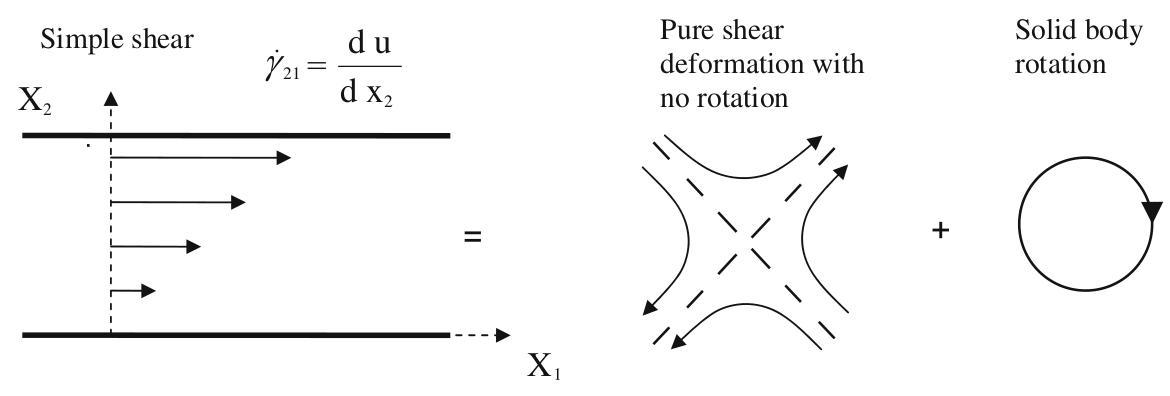
\includegraphics[width=.7\textwidth]{shear.png}
\caption{Simple shearing flow, combination of pure shear and rotation}
\end{figure}

The rotation (spin motion) does not give any contribute to the chain stretching indeed the strain rate 
tensor could be expressed in terms of the product of its eigenvalues for its eigenvectors~\cite{collins}. 

\begin{equation}
\varepsilon_{ij} \vec{\lambda} = \lambda_i \vec{\lambda_i} \qquad  i=1,2,3
\end{equation}
Since 

\[
\lambda_1 > \lambda_2 > \lambda_3 \quad \text{and} \quad \lambda_1 + \lambda_2 + \lambda_3 = 0
\]

And knowing that $\lambda_1 > 0 $ always, considering a polymer of length $= l$ we can say that the stretching phenomena happens when: % the order of interpolation that are computed during the iteration.

\begin{equation}
\vec{\lambda_1} \cdot \vec{l} \neq 0         
\end{equation}
\begin{equation}
\frac{\vec{\lambda_1} \cdot \vec{l}}{|\lambda||l|} = \cos\theta \neq 0 
\end{equation}

It is very important to know the eigenvectors and the $\cos\theta$. When we have
$\cos\theta \pm 1 $, the polymer stretching is maximum.





\subsection{Polymer solution}

As said in the introduction,~\ref{chap_introduction}, we deal with polymer-liquid systems.
In order to describe the polymer solutions at all concentration and temperatures we can refer to the phase diagram reported in figure~\ref{fig:sol} 

\begin{figure}[h]
\centering 
\includegraphics[width=.55\textwidth]{solution.png}
\caption{Phase diagram of polymer solutions}
\label{fig:sol}
\end{figure}

Considering the phase diagram, we are now interested in the dilute good solvent and dilute theta solvent.

\subsubsection{Theta solvent}
The theta solvent is the most common case for polymer solution. The $\theta$-temperature separates the poor solvent (bottom) half of the diagram from the good solvent (top) half. At this special temperature ($T=\theta$) the interaction parameter $\chi = 1/2$ and the excluded volume (see \textit{Real Chain} in~\cite{pp})
\begin{equation}
v = (1-2\chi) b^3 = \frac{T-\theta}{T}b^3 = 0
\label{eq:exvol}
\end{equation}

where $v$ is the excluded volume, and $b^3$ is the steric repulsion between monomers.
At the $\theta$-temperature the chains have nearly ideal conformation at all concentrations.

\subsubsection{Good solvent}
The upper part of the phase diagram Fig.~\ref{fig:sol} corresponds to ``good solvent''.
At lower concentration (dilute solution), polymer are far from each other and behave as isolated real chain.
At temperatures for which the excluded volume interaction within each chain exceed the thermal energy $kT$ they begin swelling.

At higher concentrations, chain interpenetrate and the solution is called semidilute. The polymer volume fraction in semidilute solution is still very low $\phi^{*} < \phi \ll 1$. 


So far all the simulations were done considering a single polimer chain in a good dilute solution. 




\subsection{Direct Numerical Simulation}\label{sec:dns}

When we deal with microscale of turbulence, in order to get a correct prediction of the Flow Field and 
the Hydrodynamic interaction, liquid-polymer chain a fully resolved flow field is required.
The Direct Numerical Simulations (DNS) is the more suitable approach.
It consists of solving the full non-linear, time-dependent Navier-Stokes equations without any empirical closure assumptions.
This means that the whole range of spatial and temporal scales of the turbulence must be resolved.
All the spatial scales of the turbulence must be resolved in the computational mesh, from the smallest dissipative scales (Kolmogorov scales)~\cite{dns,pope}, up to the integral scale $L$, associated with the motions containing most of the kinetic energy. The Kolmogorov scale, $\eta$, is given by:
\begin{equation}
\eta = \left( \frac{\nu^3}{\varepsilon} \right)^{1/4}
\label{eq:kscale}
\end{equation}
To satisfy these resolution requirements, the number N of points along a given mesh direction with increments h, must be: 
\begin{equation}
Nh > L
\label{cond1}
\end{equation}
So that the integral scale is contained within the computational domain, and also
\begin{equation}
h\leq\eta
\end{equation}
So that the Kolmogorov scale can be resolved. Since
\begin{equation}
\varepsilon \approx u'^3/L
\end{equation}

where $u'$ is the root mean square (RMS) of the velocity, the previous relations imply that a three-dimensional DNS requires a number of mesh points  $N^3$ satisfying 
\begin{equation}
N^3 \ge \mathcal{R}e^{9/4}
\end{equation}
where $\mathcal{R}e$ is the turbulent Reynolds number (Eq.~\ref{eq:re}) 
Hence, the memory storage requirement in a DNS grows very fast with the Reynolds number.
In addition, given the very large memory necessary, the integration of the solution in time must be done 
by an explicit method. This means that in order to be accurate, the integration must be done with a time 
step, $\Delta t$, small enough such that a fluid particle moves only a fraction of the mesh spacing $h$ in each step.

That is:
\begin{equation}
C=\frac{u'\Delta t}{h} < 1
\label{eq:courant}
\end{equation}

Where $C$ is the \textit{Courant number}.
The total time interval simulated is generally proportional to the turbulence time scale $\tau$ given by

\begin{equation}
\tau = \frac{L}{u'}
\end{equation}
Combining these relations, and the fact that $h$ must be of the order of $\eta$, the number of time-integration steps must be proportional to $L/(C\eta)$. On the other hand, from the definitions for $\mathcal{R}e$, $\eta$ and L given above, it follows that

\begin{equation}
\frac{L}{\eta} \sim \mathcal{R}e^{3/4}
\end{equation}
and consequently, the number of time steps grows also as a power law of the Reynolds number.

One can estimate that the number of floating-point operations required to complete the simulation is proportional to the number of mesh points and the number of time steps, and in conclusion, the number of operations grows as $\mathcal{R}e^3$.

\section{Resources}

\subsection{Available Computational Resources }
As described in the previous section the computational cost of DNS is very high, even at low Reynolds numbers.
Using DNS, it is possible to perform ``numerical experiments'', and extract from them information difficult or impossible to obtain in the laboratory, allowing a better understanding of the physics of turbulence.

Since their computational cost is very high to run a DNS simulation in a desktop computer so far and for almost the next decade is  impracticable. 

In order to run a DNS, a Super Computer or cluster of HPC (High performance Computer) is needed. The advantage of a super computer with respect to the cluster is that the single super computer can use multiple threads and CPU sharing its memory (RAM). 

For this purpose we can use a Super Computer, available to use from the department staff, and a univerity cluster. The Fortran90 code is not yet parallelized, so running simulation in the university cluster is counterproductive in terms of time of calculation, for this reason we used the Super Computer that presents the features reported on the table~\ref{value}.


\begin{table}[h]
\centering
\caption{Poseidona Super Computer datas}
\label{value}
\begin{tabular}{cc}
\toprule
\textbf{Component} &\textbf{type}  \\
\midrule
CPU & 4X Intel Xeon Processor E7 v3-4850   \\
    & 64 CPU and 128 threads   \\
CPU freq. &   2.80 GHz   \\ 
Cache     & 35 MB Last Level Cache\\
Bus speed & 8 GT/s QPI\\
GPU & NVidia GeForce GTX TITAN X\\
RAM memory                 & 128 GiB  \\
Hard Disk             & 4X 2.7 TiB  \\
OS           & Linux (arch x86\_64) \\ 
Distribution & Debian 9  \\ 
\bottomrule
\end{tabular}
\end{table}
Even though we can use this ``supercomputer'', the big amount of computation required makes the simulations very expensive in terms of physical time (more than 1 week for Simulation). 
This is due to the large amount of PDEquation, (Solved using Finite Volume Method, FVM) and the high accuracy of the code.  


\subsection{Rhea Fortran90 Code}\label{sec:code}

Before running simulation with the code a preliminary study about the theory behind the Polymer Physics and the Physic of Turbulence was done. 

After that the second step was with regards to the Fortran code. In order to run the simulations it is necessary to take confidence in and to understand the code.
Given the very complex structure of the code, reading and understanding the more important \textsc{SUBROUTINE}, of input and output, requires a long period of time.

The large system of dynamic \textit{non linear Partial Differential equations}  (PDE) is discretized in a Finite Volumes \textit{staggered grid} (or mesh) and solved using an explicit first order method for the time advancement, while for the space has been used a semi-implicit (Predictor corrector) scheme with the second order accuracy.  
The use of a staggered grid is the simplest way to avoid odd-even decoupling between the pressure and velocity. Odd-even decoupling is a discretization error that can occur on collocated grids and which leads to checkerboard patterns in the solutions.


The code reads all the variables parameters from a single file (\verb|rhea.i|), this file contains all the information regarding the operating condition and the initial-boundary condition, the order of interpolations that
is computed during the iteration, the way to solve the algebraic system that comes from the Finite Volume discretization of the equation. 
As said in the previous section, the way used to resolve the Turbulence Flow is the Direct Numerical Simulation (DNS). The code is highly accurate, because it does not model anything along the Kolmogorov eddies scale. 
Another features of this code is that it works with dimensionless magnitudes.
At the moment the code is developed just for considering a isotropic and homogeneous turbulence and periodic boundary condition.  





